% Gerado de CSVs agregados; dados numericos incorporados para portabilidade.
% Notebook SHA-256: e8ce396c21be212f5a12d673622adf543234983c3cd142088ea2dbe8e7621004
% Parecer SHA-256: 1ee24339005b98f24afb2375d080f1aaa8ff1ab0e8812427b8b103b890cef98a
% Requer: pgfplots, biblioteca statistics (somente taxas.tex).
% Ajuste opcional no chamador: \def\AlturaGrafico{4.4cm} e \def\LarguraGrafico{\linewidth}.
\begingroup
\providecommand{\AlturaGrafico}{4.4cm}
\providecommand{\LarguraGrafico}{\linewidth}
\definecolor{grafverde}{HTML}{24574D}
\definecolor{grafazul}{HTML}{1769A5}
\definecolor{grafgrafite}{HTML}{253A40}
\definecolor{graflaranja}{HTML}{B97736}
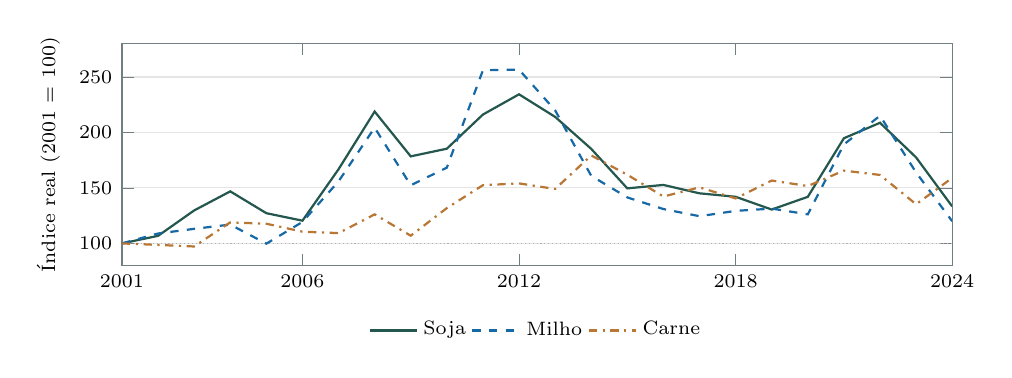
\begin{tikzpicture}
\begin{axis}[width=\LarguraGrafico,height=\AlturaGrafico,
font=\scriptsize,tick label style={font=\scriptsize},
label style={font=\scriptsize},
axis line style={grafgrafite!65},tick style={grafgrafite!65},
grid style={black!10},
legend style={font=\scriptsize,draw=none,fill=none,cells={anchor=west}},
/pgf/number format/use comma,
xmin=2001,xmax=2024,ymin=80,ymax=280,
xtick={2001,2006,2012,2018,2024},ytick={100,150,200,250},
scaled x ticks=false,xticklabel style={/pgf/number format/1000 sep=},
ymajorgrids=true,ylabel={\'Indice real (2001 = 100)},
legend columns=3,legend style={at={(0.5,-0.20)},anchor=north},
]
\addplot[black!30,densely dotted,forget plot] coordinates {(2001,100) (2024,100)};
\addplot[grafverde,thick,solid,no marks] coordinates {(2001,100.0000000000) (2002,106.8290732597) (2003,129.7117249281) (2004,146.9069763879) (2005,127.2378249174) (2006,120.4844300888) (2007,166.8318467877) (2008,218.8594646600) (2009,178.4591575935) (2010,185.3568891076) (2011,216.1428785961) (2012,234.3743788098) (2013,214.0360991498) (2014,185.2254487202) (2015,149.5971115163) (2016,152.7121258100) (2017,145.1431452906) (2018,142.0389994820) (2019,130.5314953683) (2020,141.9844369982) (2021,194.7813080281) (2022,208.7129059518) (2023,177.4885912974) (2024,133.3578613041)};
\addlegendentry{Soja}
\addplot[grafazul,thick,dashed,no marks] coordinates {(2001,100.0000000000) (2002,108.9311091293) (2003,113.1334925479) (2004,116.9792709047) (2005,99.7806603170) (2006,119.3350954823) (2007,155.9036074226) (2008,204.3366638623) (2009,152.3856266710) (2010,168.2986028315) (2011,256.0544345099) (2012,256.6122596652) (2013,219.9505085100) (2014,160.9161540693) (2015,141.4483008255) (2016,130.9809176463) (2017,124.5230137193) (2018,129.3172314256) (2019,131.3674275253) (2020,126.2060401501) (2021,189.1878054158) (2022,215.0929562744) (2023,163.9505286597) (2024,120.0016960720)};
\addlegendentry{Milho}
\addplot[graflaranja,thick,dashdotted,no marks] coordinates {(2001,100.0000000000) (2002,98.6555269731) (2003,97.2413579263) (2004,118.9469679035) (2005,117.7310104897) (2006,110.5633897398) (2007,109.2941157898) (2008,126.1821158398) (2009,106.9681582852) (2010,131.8237306951) (2011,152.4882865556) (2012,154.0790058149) (2013,149.0635684869) (2014,179.3000325991) (2015,161.8834998043) (2016,142.2702304421) (2017,150.5115941347) (2018,140.5315195989) (2019,156.6631481360) (2020,151.7037993815) (2021,165.6229252533) (2022,161.7078089666) (2023,135.2951361158) (2024,158.9944278889)};
\addlegendentry{Carne}
\end{axis}
\end{tikzpicture}
\endgroup
